\documentclass[uplatex,dvipdfmx]{beamer}
\usepackage{listings,jvlisting}
\usepackage{color}
\usepackage{xr}

\lstset{
  backgroundcolor=\color[rgb]{0.9,0.9,0.9},
  frame=single,
  basicstyle=\ttfamily
}
\makeatletter
\newcommand*{\addFileDependency}[1]{% argument=file name and extension
  \typeout{(#1)}
  \@addtofilelist{#1}
  \IfFileExists{#1}{}{\typeout{No file #1.}}
}
\makeatother

\newcommand*{\myexternaldocument}[1]{%
    \externaldocument{#1}%
    \addFileDependency{#1.tex}%
    \addFileDependency{#1.aux}%
}
\myexternaldocument{../categoryTheoryIntro/CategoryTheoryIntro}

\newcommand{\pr}[1]{\colorbox[rgb]{0.9,0.9,0.9}{\lstinline{#1}}}
\newcommand{\functype}[2]{\pr{#1 -> #2}}
\newcommand{\refcti}[1]{\cite{cti}\ref{#1}}
\newcommand{\fpmor}[3]{\pr{#1 :: #2 -> #3}}
\usefonttheme[onlymath]{serif}

\usepackage{tikz}
\usepackage{bbm}
\usepackage{amsmath,amssymb}
\usepackage{url}
\usetikzlibrary{matrix,arrows}

\newcommand{\cat}[1]{\mathbbm{#1}}
\newcommand{\arrow}{\rightarrow}
\newcommand{\functor}[3]{#1:\cat{#2}\arrow \cat{#3}}
\newcommand{\profunctor}[3]{#1:\cat{#2}\nrightarrow \cat{#3}}

\newcommand{\nat}[3]{#1:#2\Rightarrow #3}
\newcommand{\natf}[5]{#1:#2\Rightarrow #3:\cat{#4}\arrow \cat{#5}}
\newcommand{\tuple}[1]{\langle #1\rangle}
\newcommand{\objr}[1]{\mathrm{Obj}(#1)}
\newcommand{\obj}[1]{\mathrm{Obj}(\cat{#1})}
\newcommand{\morset}[1]{\mathrm{Mor}(\cat{#1})}

\newcommand{\mor}[3]{#1:#2\arrow #3}
\newcommand{\dom}{\mathrm{dom}}
\newcommand{\cod}{\mathrm{cod}}
\newcommand{\arset}[3]{\cat{#1}(#2,#3)}
\newcommand{\arsetr}[3]{#1(#2,#3)}
\newcommand{\pcobj}[1]{[#1]}
\newcommand{\funccat}[2]{\cat{#2}^\cat{#1}}

\newcommand{\coend}[2]{\displaystyle\int^{#2:\cat{#1}}\!\!\!\!\!\!\!}
\newcommand{\cend}[2]{\displaystyle\int_{#2:\cat{#1}}\!\!\!\!\!\!\!}
\newcommand{\natlat}[3]{\{#1\}_{#3\in #2}}
\newcommand{\inset}[2]{[#1,#2]}
\newcommand{\incat}[2]{[\cat{#1},\cat{#2}]}
\newcommand{\incatp}[2]{[#1,#2]}

\newenvironment{mydescription}
{\begin{description}
  \setlength{\parskip}{0.5cm}
}
{\end{description}}
\title{プロファンクターオプティクスの理論と実装}
\author{\input{../myname}}
\usetheme{Madrid}
\setbeamertemplate{navigation symbols}{}
\begin{document}
  \begin{frame}
    \titlepage
  \end{frame}
  \begin{frame}\frametitle{目的}

    データへのアクセサの一般化であるLensやキャストの一般化であるPrismは更にOpticsという概念へと一般化される。\\
    \vspace{\baselineskip}

    これらの一般化には圏論が用いられるが、圏論は自身を抽象化できることが多く。Opticsに関する議論を更に高度な圏論で一般化できると考えた。\\
  \end{frame}
  \begin{frame}\frametitle{全体の構成}
    \begin{itemize}
      \item 最初に導入として比較的身近なLensとPrismを紹介し、Opticを定義してOpticがそれらの一般化であることを示す。\\
      \vspace{\baselineskip}
      \item 次に丹原加群を定義して、Opticとの関係性を丹原Double圏同値として示す。\\
      \vspace{\baselineskip}
      \item そして最後にこれらの主要な結果として、Opticの別の形態を与えるプロファンクターの表現定理を述べる。
    \end{itemize}
  \end{frame}
  \begin{frame}\frametitle{データアクセサの一般化Lens}
    \begin{definition}[Lens]
      Lensは以下の二つの写像で構成される。
      \[\mor{\mathrm{get}}{S}{A},\ \mor{\mathrm{set}}{S\times A'}{S'}\]
    \end{definition}
    ここで$S:=B\times A,\ S':=B\times A'$とすると、
    \begin{alignat*}{7}
      \mathrm{get}:\ &S\ &\longrightarrow \ &A \ \ \ &\mathrm{set}:\ &S\times A'\ &\longrightarrow \ &S'\\
      &\tuple{b,a}&\longmapsto\ &a      &&\tuple{\tuple{b,a},a'}&\longmapsto\ &\tuple{b, a'}
    \end{alignat*}
    またこのような二つの写像の組の全体を$\mathrm{Lens}(A,A',S,S')$とする。すなわち\[\mathrm{Lens}(A,A',S,S') := \inset{S}{A}\times \inset{S\times A'}{S'}\]となる。($\inset{A}{B}$は集合$A$から$B$への写像の集合とする。)
  \end{frame}
  \begin{frame}\frametitle{キャストの一般化Prism}
    \begin{definition}[Prism]
      Prismは以下の二つの射で構成される。
      \[\mor{\mathrm{downcast}}{S}{S' + A},\ \mor{\mathrm{upcast}}{A'}{S'}\]
    \end{definition}
    ここで$S:=B+ A,\ S':=B+ A'$とすると、
    \begin{alignat*}{20}
      \mathrm{downcast}:\ &S\ \ &\longrightarrow \ \ &S'+&A & \ \ \ \ \mathrm{upcast}: &A'&\longrightarrow &\ S'\\
      &a \ \ &\longmapsto \ \ &&a &&a'&\longmapsto &a'\\
      &b \ \ &\longmapsto \ \ &b& &
    \end{alignat*}
    Lensと同様に\[\mathrm{Prism}(A,A',S,S') := \inset{S}{S'+A}\times\inset{A'}{S}\]とする。
  \end{frame}
  \begin{frame}\frametitle{Opticの定義}
    \begin{definition}[Optic]
      四つの集合$A,A',S,S'$に対するOpticの集合を\[\mathrm{Optic}(A,A',S,S') := \int^M \inset{S}{M\otimes A}\times \inset{M\otimes A'}{S'}\]と定義する。
    \end{definition}
    \begin{mydescription}
      \item[モノイダル積$\otimes$] 直積$\times$、直和$+$の一般化で集合のみならず写像のモノイダル積も取ることができる。つまり二つの写像$\mor{f}{A}{B},\ \mor{g}{C}{D}$を合成した写像
      \[\mor{f\otimes g}{A\otimes C}{B\otimes D}\]が得られる。
      \item[コエンド$\int^M$] 対象を添字とする直和集合
    \end{mydescription}
  \end{frame}
  \begin{frame}\frametitle{LensはOpticである}
    写像$\tuple{\mathrm{get},\mathrm{id}}\mor{}{S}{S\times A}$を\[\tuple{\mathrm{get},\mathrm{id}}(s)=\tuple{\mathrm{get}(s),s}\]と定義する。

    すると、$\tuple{\tuple{\mathrm{get},\mathrm{id}},\mathrm{set}}\in \inset{S}{S\times A}\times \inset{S\times A'}{S'}$となるから\[\tuple{\tuple{\mathrm{get},\mathrm{id}},\mathrm{set}}\in \int^{M}\inset{S}{M\times A}\times \inset{M\times A'}{S'}\]である。これによってLensがOpticの一種であることが分かる。\\
    \vspace{\baselineskip}
    またPrismの場合も同様に、写像$\mor{\tuple{\mathrm{\mathrm{upcast},id}}}{A'+S'}{S'}$を構成すれば簡単に示せる。
  \end{frame}
  \begin{frame}
    \frametitle{集合の圏}
    集合と写像の全体は圏と呼ばれる構造を持ち、これを$\cat{Set}$とする。\\
    \vspace{\baselineskip}
    \begin{definition}[集合の圏]
      {\small
      \begin{description}
        \item[対象] 任意の(小さい)集合を$\cat{Set}$の対象とする。
        \item[射] 対象$A,B$に対する射を任意の写像$\mor{f}{A}{B}$とする。
        \item[射の合成] 射の合成$f\circ g$はそのまま写像の合成とする。
      \end{description}
    }
    \end{definition}
  \vspace{\baselineskip}

  写像の集合は$\inset{A}{B}$で表せるが、これをOpticの集合$\mathrm{Optic}(A,A',S,S')$と置くと同様に圏が定義できる。
  \end{frame}
  \begin{frame}
    \frametitle{Opticの圏}
    \begin{definition}[Opticの圏]
      集合の圏上のOpticの圏を以下のように構成する。
      {\small
      \begin{description}
        \item[対象] 任意の(小さい)集合のニつ組を対象とする。
        \item[射] 対象$(A,A'),\ (S,S')$による射集合を$\mathrm{Optic}(A,A',S,S')$とする。
        \item[射の合成] 二つのOptic $\tuple{l',r'},\ \tuple{l,r}$の合成を$\tuple{(N\otimes l)\circ l',r'\circ(N\otimes r')}$とする。
      \end{description}
    }
    \end{definition}
    \begin{center}
      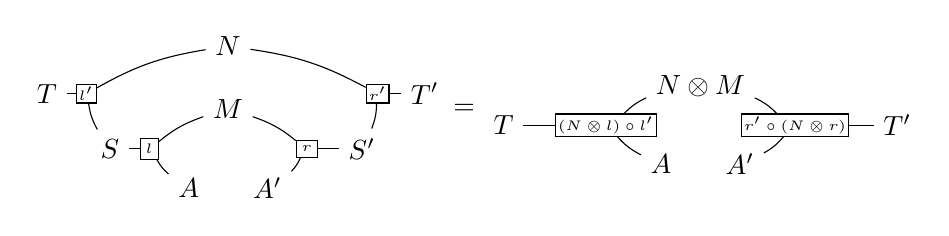
\begin{tikzpicture}
        \node (T) at (-0.8, 0.7) {$T$};

        \node (S) at (0, 0) {$S$};
        \node (M) at (1.5, 0.5) {$M$};
        \node (A) at (1, -0.5) {$A$};
        \node (N) at (1.5, 1.3) {$N$};

        \node[draw,inner sep=2pt] (l) at (0.5, 0) {{\tiny$l$}};

        \draw[-] (S) to (l);
        \draw[-] (l) to [bend left=10] (M);
        \draw[-] (l) to [bend right=10](A);
        \node[draw,inner sep=1pt] (l') at (-0.3, 0.7) {{\tiny$l'$}};
        \draw[-] (T) to (l');
        \draw[-] (l') to [bend right=10](S);
        \draw[-] (l') to [bend left=10] (N);

        \node (T') at (4, 0.7) {$T'$};
        \node (S') at (3.2, 0) {$S'$};
        \node (A') at (2, -0.5) {$A'$};
        \node[draw,inner sep=2pt] (r) at (2.5, 0) {{\tiny$r$}};
        \draw[-] (r) to (S');
        \draw[-] (r) to [bend right=10] (M);
        \draw[-] (r) to [bend left=10](A');

        \node[draw,inner sep=1pt] (r') at (3.4, 0.7) {{\tiny$r'$}};
        \draw[-] (T') to (r');
        \draw[-] (r') to[bend left=10] (S');
        \draw[-] (r') to [bend right=10] (N);

        \node (eq) at (4.5, 0.5) {$=$};

        \node (S) at (5, 0.3) {$T$};
        \node (M) at (7.5, 0.8) {$N\otimes M$};
        \node (A) at (7, -0.2) {$A$};

        \node[draw,inner sep=1pt] (l) at (6.3, 0.3) {{\tiny$(N\otimes l)\circ l'$}};
        \draw[-] (S) to (l);
        \draw[-] (l) to [bend left=10] (M);
        \draw[-] (l) to [bend right=10](A);

        \node (S') at (10, 0.3) {$T'$};
        \node (A') at (8, -0.2) {$A'$};
        \node[draw,inner sep=1pt] (r) at (8.7, 0.3) {{\tiny$r'\circ(N\otimes r)$}};
        \draw[-] (r) to (S');
        \draw[-] (r) to [bend right=10] (M);
        \draw[-] (r) to [bend left=10](A');
      \end{tikzpicture}
      \begin{tikzpicture}

      \end{tikzpicture}
    \end{center}
    またOpticの合成が定義できるので、Lens、Prismでも合成ができる。
  \end{frame}
  \begin{frame}
    \frametitle{丹原加群}

      \begin{definition}[丹原加群]
        丹原加群とは以下の図式を可換にするプロファンクター$P$と射の族\[\mor{\zeta_{A,A',M}}{P(A,A')}{P(M\otimes A, M\otimes A')}\]の組$(P,\zeta)$である。
      {\tiny
      \begin{center}
        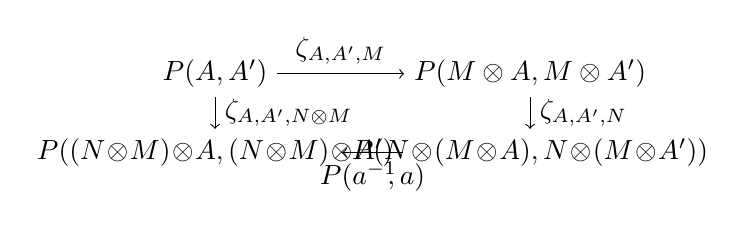
\begin{tikzpicture}[auto]
          \node (P) at (0, 0) {$P(A,A')$};
          \node (TP) at (4, 0) {$P(M\otimes A,M\otimes A')$};
          \node (TP2) at (0, -1) {$P((N\!\otimes\!M)\!\otimes\!A,(N\!\otimes\! M)\!\otimes\! A')$};
          \node (TTP) at (4, -1) {$P(N\!\otimes\! (M\!\otimes\! A),N\!\otimes\! (M\!\otimes\! A'))$};
          \draw[->] (P) to node{$\zeta_{A,A',M}$}(TP);
          \draw[->] (P) to node{$\zeta_{A,A',N\otimes M}$}(TP2);
          \draw[->] (TP) to node{$\zeta_{A,A',N}$}(TTP);
          \draw[->] (TP2) to node{$P(a^{-1}\!\!,a)$}(TTP);
        \end{tikzpicture}
        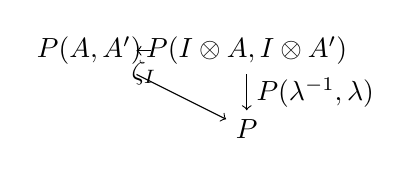
\begin{tikzpicture}[auto]
          \node (P) at (0, 0) {$P(A,A')$};
          \node (TP) at (2, 0) {$P(I\otimes A,I\otimes A')$};
          \node (P2) at (2, -1) {$P$};
          \draw[->] (P) to node{$\zeta_I$}(TP);
          \draw[->] (TP) to node{$P(\lambda^{-1},\lambda)$}(P2);
          \draw[->] (P) to(P2);
        \end{tikzpicture}
      \end{center}}
      \end{definition}
      ただし、プロファンクターは圏上の二項演算の一種である。
  \end{frame}
  \begin{frame}
    \frametitle{丹原加群の圏}
    \begin{definition}[丹原加群の圏]
      丹原加群の圏$\cat{Tamb}$を以下のように定義する。
      {\small
      \begin{description}
        \item[対象] 任意の丹原加群$(P,\zeta)$を対象とする。
        \item[射] 以下の図式を可換にする射の族$\mor{\alpha_{A,A'}}{P(A,A')}{Q(A,A')}$を射とする。\\
        {\tiny
          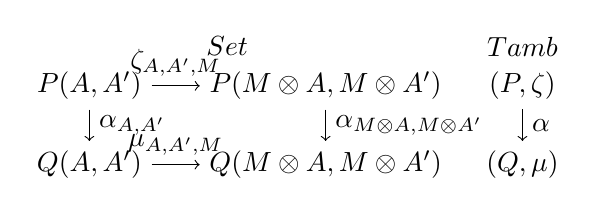
\begin{tikzpicture}[auto]
            \node (P) at (-1, 0) {$P(A,A')$};
            \node (Q) at (-1, -1) {$Q(A,A')$};
            \node (TP) at (2, 0) {$P(M\otimes A, M\otimes A')$};
            \node (TQ) at (2, -1) {$Q(M\otimes A, M\otimes A')$};
            \node (catpr) at (0.75, 0.5) {$\cat{Set}$};
  
            \draw[->] (P) to node{$\alpha_{A,A'}$}(Q);
            \draw[->] (P) to node{$\zeta_{A,A',M}$}(TP);
            \draw[->] (TP) to node{$\alpha_{M\otimes A,M\otimes A'}$}(TQ);
            \draw[->] (Q) to node{$\mu_{A,A',M}$}(TQ);
  
            \node (P) at (4.5, 0) {$(P,\zeta)$};
            \node (Q) at (4.5, -1) {$(Q,\mu)$};
            \draw[->] (P) to node{$\alpha$}(Q);
            \node (cattam) at (4.5, 0.5) {$\cat{Tamb}$};
  
          \end{tikzpicture}
          }
        \item[射の合成] 元の圏の射の合成からそのまま定義できる。
      \end{description}
      }
    \end{definition}
  \end{frame}
  \begin{frame}
    \frametitle{Opticの圏と丹原加群}
    丹原加群は$\cat{Optic}$から$\cat{Set}$への準同型写像と対応する。\\
    これは厳密には以下の定理として示せる。\\
    \vspace{\baselineskip}

    \begin{theorem}[丹原Double圏同値]
      \[\cat{Tamb}\simeq\incat{Optic}{Set}\]
      $\simeq$は圏の同型を緩めた等価性とし、$\incat{Optic}{Set}$は$\cat{Optic}$から$\cat{Set}$への準同型写像の成す圏である。
    \end{theorem}
    \vspace{\baselineskip}

    また特に示さないが既存の文献での証明は行間が広いため証明の一部を補完した。
  \end{frame}
  \begin{frame}\frametitle{プロファンクターオプティクス}
    最後に最終目標であるプロファンクターの表現定理を示す。
    \begin{theorem}[プロファンクターの表現定理]
      \[\cat{Optic}(A,A',S,S') \cong \int_P \inset{P(A,A')}{P(S,S')}\]
      ただし$P$は任意の丹原加群とする。
    \end{theorem}
    \vspace{\baselineskip}

    本来$P$は丹原加群ではなく、$\cat{Optic}$から$\cat{Set}$の準同型写像であるが、前スライドの丹原Double圏同値によって丹原加群とみなせる。\\
    \vspace{\baselineskip}
    また左辺のような形で表したOpticをプロファンクターオプティクスと呼び、実用ではこちらを用いることが多い。
  \end{frame}
  \begin{frame}
    \frametitle{まとめ}
    \begin{itemize}
      \item 丹原Double圏同値の証明の一部を補完できた。\\
      \vspace{\baselineskip}
      \item 上の定理の一般化となるように思われる定理を2-categoryに関する論文から見つけ出すことができた。
    \end{itemize}
  \end{frame}
  \begin{frame}\frametitle{今後の課題}
    \begin{itemize}
      \item 2-categoryに関する体系的な知識を身につける。\\
      \vspace{\baselineskip}

      \item 丹原Double圏同値の一貫した証明を示す。\\
      \vspace{\baselineskip}

      \item 丹原Double圏同値を2-categoryによって一般化する。
    \end{itemize}
  \end{frame}
\end{document}
